\ylDisplay{Skeem} % Ülesande nimi
{Tundmatu autor} % Autor
{lahtine} % Voor
{2009} % Aasta
{G 3} % Ülesande nr.
{4} % Raskustase
{
% Teema: Elektriahelad
\ifStatement
Elemendi $X$ takistus muutub sõltuvalt selle pingest. Kui $U_X \leq \SI{1}{V}$,
siis selle takistus on $R_1 = \SI{1}{\ohm}$, kui aga $U_X > \SI{1}{V}$, siis on takistus $R_2 =
\SI{2}{\ohm}$. Kolm elementi $X$ ühendatakse ideaalse ampermeetriga, nagu näidatud joonisel.
Väljundklemmidele rakendatakse pinge, mille ajaline sõltuvus on toodud graafikul.
Joonestage ampermeetri näidu ajalise sõltuvuse graafik.

\begin{center}
	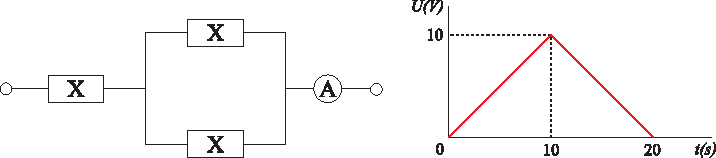
\includegraphics[width=\linewidth]{2009-lahg-03-yl}
\end{center}
\fi


\ifHint
Süsteem saab töötada kolmes erinevas režiimis. Esiteks, kui pinge on piisavalt madal või kõrge, on kõikide elementide takistus vastavalt \SI{1}{\ohm} või \SI{2}{\ohm}. Vahepealse pinge väärtuse korral on vasakpoolse elemendi takistus \SI{2}{\ohm} ja parempoolsetel \SI{1}{\ohm}. Teisi režiime ei ole, sest vasakpoolse takisti pinge on alati suurem kui parempoolsetel ning seega ei saa vasaku takisti takistus olla väiksem kui parempoolsetel.
\fi


\ifSolution
Süsteem saab töötada kolmes režiimis:\\
(I) Kõigi elementide takitus on \SI{1}{\ohm}. Siis süsteemi kogutakistus on $R_I = \SI{1,5}{\ohm}$, vool $I_I = \frac{U}{\num{1,5}}(\si{A})$ ning pinge skeemi vasakpoolsel elemendil $\frac{2}{3}U$ ja parempoolsetel elementidel $\frac 13U$.\\
(II) Vasakpoolse elemendi takistus on \SI{2}{\ohm}, parempoolsemate elementide takistus on \SI{1}{\ohm}. Siis süsteemi kogutakistus on $R_I = \SI{2,5}{\ohm}$, vool $I_I = \frac{U}{\num{2,5}}(\si{A})$ ning pinge vasakpoolsel elemendil $\frac 45U$ ja parempoolsetel elementidel $\frac 15U$.\\
(III) Kõigi elementide takitus on \SI{2}{\ohm}. Siis süsteemi kogutakistus on $R_I = \SI{3}{\ohm}$, vool $I_I = \frac U3(A)$ ning pinge skeemi vasakpoolsel elemendil $\frac 23U$ ja parempoolsetel elementidel $\frac 13U$.

Vaatame süsteemi käitumist, kui klemmipinge kasvab. Alguses töötab süsteem režiimis I kuni hetkeni, mil klemmipinge kasvab väärtuseni $U = \SI{1,5}{V}$. Siis muutub vasakpoolse elemendi takistuse väärtus $R_2 = \SI{2}{\ohm}$-ks ning süsteem jätkab tööd režiimis II. Hetkel, mil klemmipingepinge kasvab väärtuseni $U = \SI{5}{V}$, muutub ka parempoolsete elementide takistus $R_2$-ks ning süsteem jätkab tööd režiimis III.

Vaatame süsteemi käitumist, kui klemmipinge kahaneb. Alguses töötab süsteem režiimis III kuni hetkeni, mil klemmipinge langeb väärtuseni $U = \SI{3}{V}$. Siis muutub parempoolsete elementide takistuse väärtus tagasi $R_1 = \SI{1}{\ohm}$-ks ning süsteem jätkab tööd režiimis II. Hetkel, mil klemmipingepinge langeb väärtuseni $U = \SI{1,25}{V}$, muutub ka vasakpoolse elemendi takistus tagasi $R_1$-ks ning süsteem jätkab tööd režiimis I. Voolutugevuse käitumine on esitatud graafikul.

\begin{center}
	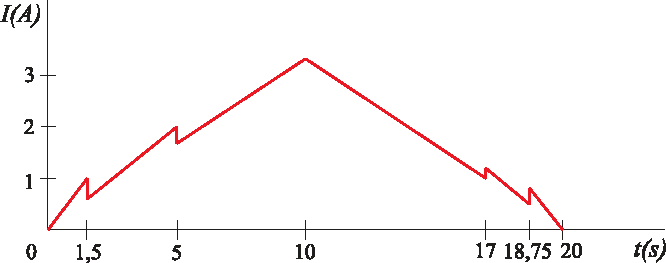
\includegraphics[width=0.9\linewidth]{2009-lahg-03-lah}
\end{center}
\fi
}